\documentclass[twoside]{article}
\usepackage{aistats2022}
% If your paper is accepted, change the options for the package
% aistats2022 as follows:
%\usepackage[accepted]{aistats2022}

% If you set papersize explicitly, activate the following three lines:
%\special{papersize = 8.5in, 11in}
%\setlength{\pdfpageheight}{11in}
%\setlength{\pdfpagewidth}{8.5in}

\let\oldsection\section
\renewcommand{\section}[1]{\oldsection{\uppercase{#1}}}

% If you use natbib package, activate the following three lines:
\usepackage[round]{natbib}
\renewcommand{\bibname}{References}
\renewcommand{\bibsection}{\subsubsection*{\bibname}}

\usepackage[utf8]{inputenc} % allow utf-8 input
\usepackage[T1]{fontenc}    % use 8-bit T1 fonts
\usepackage{hyperref}       % hyperlinks
\usepackage{url}            % simple URL typesetting
\usepackage{booktabs}       % professional-quality tables
\usepackage{microtype}      % microtypography
\usepackage{graphicx}
\graphicspath{{../figs/}{../}}
%\usepackage{subfigure}
\usepackage{subcaption}
\usepackage{hyperref}       % hyperlinks
\usepackage[dvipsnames]{xcolor}

\hypersetup{ % SLJ: my standard paper setup...
	pdftitle={MAP convergence},
	pdfkeywords={},
	pdfborder=0 0 0,
	pdfpagemode=UseNone,
	colorlinks=true,
	linkcolor=blue, %mydarkblue,
	citecolor=blue, %mydarkblue,
	filecolor=blue, %mydarkblue,
	urlcolor=blue, %mydarkblue,
	pdfview=FitH,
	pdfauthor={Anonymous},
}


\newcommand{\RLP}[1]{\textcolor{red}{RLP:#1}}
\newcommand{\fdk}[1]{\textcolor{Periwinkle}{fdk:#1}}
\newcommand{\TODO}[1]{\textcolor{cyan}{TODO #1}}

% my packages
\usepackage{../math_commands}
% some custom math commands
\newtheorem{proposition}{Proposition}
\newcommand*{\expect}[2][]{\ensuremath{\mathbb{E}_{#1} \left[ #2 \right] }} % expectation operator
\newcommand{\cond}{\,\vert\,}
\newcommand{\logpart}{A}
\newcommand{\conj}{\logpart^*}
\newcommand{\bregman}{\cB_\logpart}
\newcommand{\bregmanconj}{\cB_{\logpart^*}}
\newcommand{\natp}{\theta}
\newcommand{\meanp}{\mu}
\newcommand{\decrement}{D}
\newcommand{\linear}{\ell} % linearization of a function
\newcommand{\lr}{\gamma} % learning rate, or step-size
\newcommand{\lin}[1]{\left\langle#1\right\rangle}

\newcommand{\MAPm}{\hat \mu_n}
\newcommand{\MAPt}{\hat \natp_n}



\begin{document}

% If your paper is accepted and the title of your paper is very long,
% the style will print as headings an error message. Use the following
% command to supply a shorter title of your paper so that it can be
% used as headings.
%
%\runningtitle{I use this title instead because the last one was very long}

% If your paper is accepted and the number of authors is large, the
% style will print as headings an error message. Use the following
% command to supply a shorter version of the authors names so that
% they can be used as headings (for example, use only the surnames)
%
%\runningauthor{Surname 1, Surname 2, Surname 3, ...., Surname n}

\twocolumn[

\aistatstitle{Looking for Convergence Rates\\ for the MAP of the Exponential Family}


\aistatsauthor{R\'emi Le Priol \And Frederik Kunstner \And  Damien Scieur \And Simon Lacoste-Julien }

\aistatsaddress{ Mila \And  UBC \And SAIT SAIL \And Mila} 
]

\begin{abstract}
We consider the problem of upper bounding the expected sub-optimality of the maximum likelihood estimate (MLE), or a conjugate maximum a posteriori (MAP) for the exponential family. 
Surprisingly, we found no solution to this problem in the literature -- e.g. after seeing 5 samples, we do not know how many bits away (in expectation) our model is from the true distribution.
After displaying some properties and special cases of this problem, 
we show it is an application of several optimization algorithms.
Yet it falls out of scope for current analysis, thus highlighting areas for progress.
\end{abstract}

\section{Motivation}

We kind of know how to do optimization 
on smooth, strongly convex functions 
when there is some bound on the stochasticity,
for example in the form of a bounded variance, 
say for the problem 
\begin{equation}
\min_\theta f(\theta)
\end{equation}
with access to stochastic gradients 
$g(\theta)$ such that 
\begin{equation}
	\expect{\norm{g(\theta) - \nabla f(\theta)}^2} \leq \sigma^2.
\end{equation}
Estimating the mean of Gaussian noise is a special case of this problem class, using 
$f(\theta) = \frac{1}{2}\norm{\theta - \mu}^2$ and $g(\theta) \sim \cN(\theta - \mu, \sigma^2)$.
SGD with a decreasing step-size coincides with the maximum likelihood estimate (MLE), 
and attains the $1/t$ convergence rate.

But our understanding of stochastic optimization lacks in other domains. 
A generalization of the above problem, at the intersection of optimization and statistics, 
is the problem of minimizing 
\begin{equation}
	f(\theta) = \expect[x \sim p(x\cond\theta_*)]{-\log p(x\cond\theta_*)},
\end{equation}
When $p(x\cond\theta)$ is an exponential family distribution,
$-\log p(x\cond\theta) = A(\theta) - \lin{t(x), \theta}$ (up to constants).
Here, $A$ is the log-partition function, a Legendre function that we assume can be minimized in closed form.
The Gaussian example is the special case $A(\theta) = \frac{1}{2}\norm{\theta}^2$.

There are algorithms for this setting, for example the MLE;
giving the (online) maximum likelihood after seeing $t$ samples
corresponds to online mirror descent with decreasing step-sizes (more on this later).
But our convergence rates are weak; they are either asymptotic, cover only special cases or require having seen many ($n \gg d$) samples.

We do not have a solution. The goal of this paper, and the reason it is submitted at AISTATS, 
is to bring this issue to the attention of the community working at the intersection of machine learning, optimization and statistics,
in the hope that we can make progress on this question;
Can we build algorithms for stochastic estimation 
when the objective function is not (close to) quadratic
and the noise is not Gaussian?

We show the connections between the optimization and statistical estimation view of the problem
and discuss where our current theory fails to fully capture the problem.
We are aware that \emph{a} solution to this problem would be the maximum likelihood estimate---this is part of the point of this paper---and 
that the statistical theory results for the convergence of the MLE to the solution are well known. 
Our point is more subtle, in that for the purposes of optimization, to mimic the results that are known for SGD in Euclidean settings, 
we would like a result of the form 
\begin{equation*}
	\text{optimality gap after $t$ steps}
	\leq 
	\frac{\text{``bias''}}{t^2}
	+ \frac{\text{``variance''}}{t},
\end{equation*}
which is the bit that is lacking. 

% Then; 
% - description of the setting
% - statistical solutions (asymptotic, l1 or l2 error)
% - optimization solutions (online+bounded gradient, self-concordance, more recent relative smoothness results)
% - potential application of ideas that would solve this, beyond this problem (acceleration, causality?)
% - conclusion?


\section{Technical background}

\RLP{Goal = disseminate related work to make it look nice.}
Exponential Families are an elegant and lean way to model a wide variety of data : binary, categorical, natural numbers, positive float, long or short tailed... 
They are literally the linear model of probabilities.
The exponential family for data $X$ with natural parameter $\natp$  is entirely specified by the support set of the data   $\cX$ and a sufficient statistic $T: \cX \rightarrow \real^d$
\begin{equation}
	 p(X|\natp) = \exp( \natp^\top T(X) - \logpart(\natp)) \; ,
\end{equation}
where $\logpart$ is the log-partition function -- i.e. the normalization factor
\begin{align}
    \logpart(\natp) = \log \int e^{\natp^\top T(x)} dx 
\end{align}
where the integral stands for a sum if $x$ has discrete support. \RLP{Use base measure instead.}
For instance, this simple model encompasses both categorical distributions $\cX = \{1, \dots, k\}$ with $T(X)$ being the one-hot encoding, and multivariate normal distributions $\cX=\real, T(X)=(X, X^2)$. 

\paragraph{Duality}
The logpartition function $\logpart$ verifies the two following identities
\begin{align}
    \nabla\logpart(\natp) &=  \expect[p(X|\natp)]{T(X)} =: \meanp \\
    \nabla^2 \logpart(\natp) &= \Cov_\natp[T(X)] > 0
\end{align}
where $\meanp$ is called the mean parameter.
If the sufficient statistic $T$ is minimal, then the log-partition function $\logpart$ is strictly convex and its gradient $\nabla \logpart$ is a bijection between natural parameters $\natp$ and mean parameters $\mu$.
We will write indifferently $\mu$ or  $\natp$ depending on the context, being aware that both represent the same distribution.
The second identity entails that $\logpart$ is strictly-convex. 
At this point it is useful to introduce the \href{https://en.wikipedia.org/wiki/Convex_conjugate}{convex conjugate} (aka Fenchel-Legendre transform) of the logpartition function
\begin{align}
	\conj(\mu) = \langle \mu, \natp \rangle - \logpart(\natp) \; .
\end{align}
which matches the common notion of \textit{entropy} in information theory.
If $\logpart$ is strictly convex, then its gradient is strictly monotone, so it is a bijection, and its inverse is the gradient of its dual $\nabla\conj \circ \nabla\logpart(\natp) = \natp$ (cf Fig.~\ref{fig:duality}).
For a full review of exponential families and their duality, see \citet[Chapter 3]{wainwright2008graphical}.
\begin{figure}[ht]
	\centering
	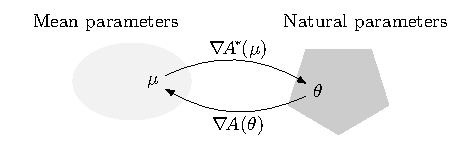
\includegraphics{duality}
	\caption{The gradient of the log-partition function and its dual, $(\nabla \logpart, \nabla \conj)$, form a bijection between the natural and mean parameters $\natp, \meanp$. Figure reproduced from \citet{kunstner2020homeomorphic}.
		\RLP{Show the true gaussian bijection instead?}
	}
	\label{fig:duality}
\end{figure}

\paragraph{Bregman Divergences}
A very useful object to keep in mind is the Bregman divergence induced by $\logpart$ between two parameters $\natp$ and $\natp_0$
\begin{align}
    \bregman (\natp ; \natp_0)
    & = \logpart(\natp) - \logpart(\natp_0) 
    - \langle \nabla \logpart(\natp_0)  , \natp - \natp_0 \rangle
\end{align}
with $\nabla \logpart(\natp_0) = \expect[\natp_0]{T(X)} =: \meanp_0$ the mean parameter associated to $\natp_0$. 
It is a non-symmetric measure of distance between parameters.
It is equal to the divergence of its convex conjugate with switched arguments
\begin{align}
	\bregman (\natp ; \natp_0)
    = \bregmanconj ( \meanp_0 ; \meanp) \; .
\end{align}

\paragraph{Conjugate Prior}
One conjugate prior \citep{agarwal2010geometric} for $p(X|\natp)$ is
\begin{align}
    p(\natp) &\propto \exp( - n_0 \bregman(\natp ; \natp_0) )
\end{align}
where $n_0$ and $\natp_0$ are (hyper)parameters of the prior, and $\bregman(\natp ; \natp_0)$ is introduced above.
Intuitively, $n_0$ is a number of fictive points observed from a distribution with parameter $\natp_0$.
The negative log-likelihood of the prior is
\begin{align*}
    -\log p(\natp) = n_0 (\logpart(\natp)  - \natp^\top \meanp_0 ) + \cst
\end{align*}
which is the formula for the exponential family with sufficient statistics $(\natp ,\logpart(\natp))$ and with natural parameter $(n_0 \mu_0, -n_0)$.
Then the joint log-likelihood of $\cD =(X_1,\dots,X_n,\natp)$ is
\begin{multline}
    -\log p(\cD|\natp)p(\natp) 
    = (n_0+n) \logpart (\natp) \\
    - \theta^\top \left(n_0 \meanp_0 + \sum_{i=1}^n T(X_i) \right) + \cst
    \label{eq:joint_likelihood}
\end{multline}
meaning the posterior given $\cD=(X_1,\dots, X_n)$ is part of the same family, with natural parameters $(n_0 \mu_0 + \sum_i T(X_i) , -(n_0 + n))$.

\paragraph{Maximum A Posteriori (MAP).}
Minimizing~\eqref{eq:joint_likelihood} over $\natp$ yields the MAP estimate
\begin{align}
    \hat \natp = \argmin_\natp -\log p(\cD|\natp) + n_0 \bregman(\natp ; \natp_0)
\end{align}
verifying the first oder optimality conditions \RLP{$\natp$ unconstrained, living in an open set with barriers}
\begin{align}
    \nabla \logpart(\hat \natp_\text{MAP}) = \hat \meanp_\text{MAP}
    = \frac{n_0 \meanp_0 + \sum_{i=1}^n T(X_i) }{n_0+n} \; .
\end{align}
When $n_0=0$ -- eg we observed zero samples from the prior -- we recover the Maximum Likelihood Estimate (MLE)
\begin{align}
	\hat \mu_\text{MLE} = \frac{\sum_{i=1}^n T(X_i)}{n}
\end{align}
These rules are known as moment matching.
The MLE and MAP estimates are statistics of the dataset $\cD$. Given a random dataset, we wish to bound their deviation from the optimum $\natp^*$ or $\meanp^*$.


\section{Open Problem}

\fdk{
Might want to note that a perhaps ``typical'' view of parameter estimation 
works with norms, e.g. bounding $\expect[p(x\cond\theta_*)]{\norm{\theta-\theta_*}^p}$ (for some norm and some power), 
or more generally using distances rather than divergences as they are symmetric and have nicer properties. 
But as the MLE is the minimizer of the log-likelihood, 
using the log-likelihood (and by extension the KL divergence) as a measure of risk is natural, if inconvenient.
}


For a well-specified model, the suboptimality on the population log-likelihood is exactly the KL between our current model and the true distribution
\begin{multline}
    \expect[X\sim p(.|\natp^*)]{-\log p(X|\natp) + \log p(X|\natp^*) } \\
	= \KL( p(.|\natp^*) ; p(.|\natp)) \; .
\end{multline}
For the exponential family, the KL is equal to the Bregman divergence induced by the log-partition function, or alternatively by the entropy, being careful with the order of the arguments 
\begin{align}
\boxed{
	\KL( p(.|\natp^*) ; p(.|\natp))
    = \bregman (\natp ; \natp^*)
    = \bregmanconj ( \meanp^* ; \meanp)
}
\end{align}
Our question is: how does this quantity behave when $\natp$ is the maximum-likelihood or the MAP estimate ? Can we get upper-bounds on the following quantities
\begin{align}
	\label{eq:bregmanMLE}
	\expect[\cD]{\bregmanconj \left (\E [T(X)] ;  \inv{n}  \smallsum_i T(X_i) \right )} \\
	\label{eq:bregmanMAP}
	\expect[\cD]{\bregmanconj \left (\E [T(X)] ; \frac{n_0 \mu_0 + \smallsum_i T(X_i)}{n_0+n} \right )} 
\end{align}
where the outer expectation is on the dataset $\cD = \{X_1, \dots, X_n \}$ sampled i.i.d as $X_i\sim \natp^*$?
More explicitly, can we write an upper bound that does not involve an expectation over the dataset -- e.g. where the stochasticity is removed.


\paragraph{Remark.}
This could be seen as a concentration inequality, expressed with a Bregman divergence instead of a norm.
A key difference though, is that the random variable $T(X)$ is connected to the metric $\logpart$. 
Indeed expressions~\eqref{eq:bregmanMLE} or~\eqref{eq:bregmanMAP} can be infinite for another choice of random variable. 
For instance, if we plug in $\conj(\mu)= -\log(\mu)$, which defines a divergence on positive numbers, and $T(X) \sim \cN(0,1)$ which can be negative.

\paragraph{Remark 2.}
The expectation of the MLE may be infinite, for instance with $\cN(0,\sigma^2)$ and $n\leq 2$. Instead of taking the expectation,  we might want to bound this quantity in high probability, without resorting to Markov inequality, but that is a difficult endeavor.

\section{Insight - Asymptote}
As a reference point for any finite convergence rate, it is interesting to know the asymptotic behavior of these quantities as $n \rightarrow +\infty$.
We can get the asymptote by approximating the Bregman divergence using a second order Taylor expansion
\begin{align}
    \bregmanconj(\mu^* ; \mu) 
    &=\half  \norm{\mu^* - \mu}^2_{\nabla^2\conj(\mu^*)}
    + O(\norm{\mu - \mu^*}^3)
\end{align}
where the norm  $\| x \|_\mM^2 = x^\top \mM x$  is induced by the hessian at the optimum 
\begin{align}
    \nabla^2\conj(\mu^*) 
    = \nabla^2\logpart(\natp^*)^{-1} 
    = \Cov_{\natp^*}[T(X)]^{-1}  \; .
\end{align}
Both the MLE and the MAP have the same asymptotic rate
\begin{align}
\label{eq:MAP_asymptote}
	\E \bregmanconj \left (\E [T(X)] ;  \frac{n_0 \mu_0 + \smallsum_i T(x_i)}{n_0+n} \right ) 
	= \frac{d}{2n} + O(n^{- \frac{3}{2}})
\end{align}
as the contribution of the prior $n_0 \meanp_0$ gets negligible compared to the data.
Remark how this rate is also independent of the optimum $\meanp^*$.
\fdk{meaning "independent ignoring constants"?}

\fdk{
That should be well known, maybe find a reference?
% Something about the statistical asymptotic behavior for the MLE? 
% \begin{equation}
% 	D_A(\theta_*, \theta_n) \approx \frac{1}{2}\norm{\theta_n - \theta_*}_{\nabla^2 A(\theta_*)}^2 
% 	\approx \frac{1}{n}?
% \end{equation}
}

\section{Example - Gaussian Mean}

\paragraph{$\ell^2$-norm Analysis}
In the Euclidean realm, the average is bounded by variance becomes a bound on the variance of the average
\begin{align}
	\Var T(X) = \E \norm{T(X) - \mu^*}^2 = \sigma^2 \\
	\implies \E \norm{\mu^* -  \inv{n}  \smallsum_i T(x_i)}^2 = \frac{\sigma^2}{n} 
\end{align}
eg the variance of the mean is $n$ times smaller than the variance of the samples.
Adding a reference mean $\mu_0$ to get the MAP yields
\begin{align}
	\E \norm{\mu^* -  \frac{n_0 \mu_0 + \smallsum_i T(x_i)}{n_0+n} }^2 
	&= \frac{n}{(n+n_0)^2} \sigma^2 +  \frac{n_0^2}{(n+n_0)^2} \norm{\mu^* -  \mu_0}^2 \\
	&= O\left(\frac{\sigma^2}{n} \right) + O\left(\frac{\norm{\mu^* -  \mu_0}^2}{n^2} \right)
\end{align}
so we have a variance term in $O(n^{-1})$ and a bias term decreasing as $O(n^{-2})$. Let's see if we can get similar estimates for arbitrary exponential families !



\section{Insight - Euclide's World}
As another reference point, if we make restrictive assumptions on the log-partition function, we can ensure our objective will behave at least as nicely as the mean of a gaussian.
\paragraph{If $\conj$ is $L$-Lipschitz} (e.g. $\logpart$ is defined within the $\ell^2$-ball of radius $L$), then
\begin{align}
    \bregmanconj(\mu^* ; \mu) 
    &\leq L \norm{\mu^* - \mu} + \norm{\natp} \norm{\mu^* - \mu} \\
    &\leq 2L \norm{\mu^* - \mu}
\end{align}
so $\bregmanconj$ is $2L$-Lipschitz, and we get a $O(\inv{\sqrt{t}})$ convergence rate from \RLP{Gaussian rate}.
\paragraph{If $\conj$ is $L$-smooth} (e.g. $\logpart$ is $L^{-1}$-strongly convex), then
\begin{align}
    \bregmanconj(\mu^* ; \mu) 
    \leq \frac{L}{2} \norm{\mu^* - \mu}^2
\end{align}
so $\bregmanconj$ is upper bounded by a quadratic, and we get the same rate as a Gaussian.


\section{Example - Gaussian Variance}
A core example of this paper is a centered gaussian with unknown variance $\cN(0,\sigma^2)$. 
The density is	$p(x) = \inv{\sqrt{2\pi \sigma^2}} e^{-\frac{x^2}{2 \sigma^2}}$.
Defining $T(X)=X^2$ as the sufficient statistic, we get natural parameter $\natp = -\inv{2 \sigma^2} <0$, and mean parameter $\mu=\E[T(X)] = \sigma^2 >0$. 
Mean and natural parameters are roughly inverse of each other $\natp = -\inv{2 \mu}$.
Now we can match the log-likelihood with the exponential family template to get the log-partition function, and taking the conjugate to find the entropy
\begin{align}
	\logpart (\natp) &= - \half \log(-\natp)  + \half \log(\pi) \\
	\conj(\mu) &= \half\left( -\log(\mu) + \log\frac{\pi}{2} - 1 \right) \; .
\end{align}
Both the log-partition and  the entropy are roughly negative logarithm $z\mapsto - \log(z)$.
It means the conjugate prior is the exponential family with sufficient statistic $(\natp, \log(-\natp) )$, eg a negative Gamma distribution.
It also means $\bregman$ and $\bregmanconj$ have the same shape
\begin{align}
	\bregmanconj( \mu_*; \mu_n) 
	&= \half \left ( \frac{\mu_*}{ \mu_n} - 1 - \log  \frac{\mu_*}{ \mu_n} \right) \\
	\bregman( \natp_n; \natp_* )
	&=  \half \left ( \frac{ \natp_n}{\natp_*} - 1 - \log  \frac{ \natp_n}{\natp_*} \right) \; .
\end{align}
In other words, this divergence measures the discrepancy between the ratio $\frac{ \natp_n}{\natp_*} =  \frac{\mu_*}{ \mu_n}  $ and $1$ via the function $\phi$
\begin{align}
	\phi(z) := \half (z - 1 - \log(z))
\end{align}
illustrated in Figure~\ref{fig:phi}. 
Below we report upper bounds on the expected value of this divergence for the MLE and the MAP.


\begin{figure}[ht]
	\centering
	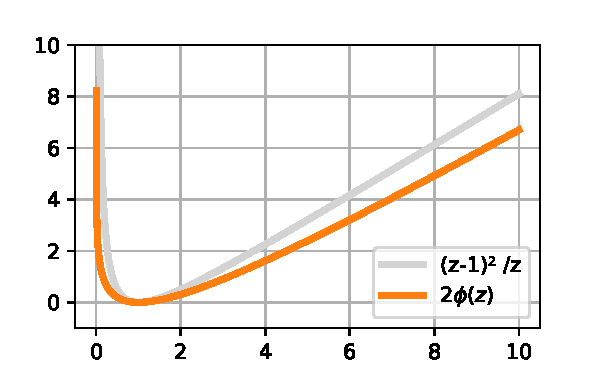
\includegraphics[width=.4\textwidth]{phi.pdf}
	\caption{$\phi(z)$ is the Bregman divergence induced by $-\log(z)$. It is a barrier near $0$. As a result, it is poorly approximated by quadratics, but it admits another upper-bound (in grey).}
	\label{fig:phi}
\end{figure}

\begin{figure}[ht]
	\centering
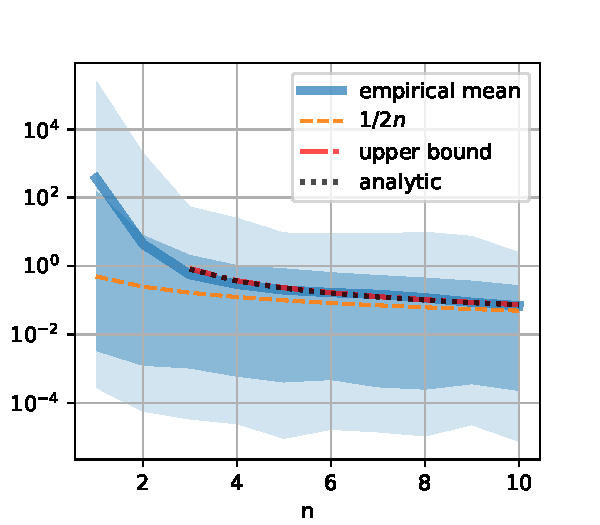
\includegraphics[width=.4\textwidth]{fewsamples.pdf}
	\caption{Suboptimality of a Gaussian variance MLE against number of samples $n$. Bold curve is average over 100 trials,  dark shaded area is 90\% (dark) confidence interval, light shade is min-max interval. 
		While the expected value is infinite for $n=1$ or $n=2$, it quickly matches the upper bound, and the $1/2n$ asymptote.
	}
	\label{fig:curves}
\end{figure}


\begin{theorem}[MLE Tight Bound]
	The MLE of $\cN(0,\mu_*)$ is $\hat \mu_n^\text{MLE} = \inv{n} \sum_i X_i^2 $.
	Its expected suboptimality is infinite when $n\leq 2$, and otherwise upper-bounded as
	\begin{align}
		 \expect{\bregmanconj( \mu_*; \hat \mu_n^\text{MLE}) }
			\leq \inv{2n} +\frac{2}{n(n-2)} \; .
			\label{eq:MLE_rate}
	\end{align}
\end{theorem}

This upper bound is asymptotically tight.
We illustrate its numerical behavior in Figure~\ref{fig:curves}.
We get a similar bound for the multivariate generalization :
the expected value is infinite whenever $n \leq d+1$ where $d$ is the dimension, and is otherwise bounded by $O(\frac{d^2}{n} + \frac{d^3}{n(n-d-1)} )$.
  
For the MAP, we get an upper bound thanks to the inequality $ - \log(z) \leq \inv{z} - 1$ which implies
\begin{align}
	\label{eq:log_bound} 
	\phi(z) \leq \half (z + \inv{z}) - 1 = \frac{(z-1)^2}{2 z} \; .
\end{align}

\begin{theorem}[MAP Bound]
 For $n\in \naturalnumbers$, let us  define
 \begin{align}
	b_n = \frac{(1 + \inv{n_0} - \frac{\mu_0}{\mu^*})^2}{2 (\frac{\mu_0}{\mu^*}+\frac{(n-2)_+}{n_0})(1 + \frac{n}{n_0} )} \; .
 \end{align}
The expected suboptimality of the MAP of $\cN(0,\mu^*)$ with prior hyper-parameters $(n_0,\mu_0)$ is
 \begin{equation}
	\expect{\bregmanconj( \mu_*; \hat \mu_n^\text{MAP})}
	\leq \begin{cases}
		\inv{2(n_0+1)}  +  b_1 \ \text{if}\ n=1,\\
		\frac{1}{n_0 \frac{\mu_0}{\mu^*} +n-2} + b_n \ \text{if}\ n\geq 2
	\end{cases}
	\label{eq:MAP_rate}
\end{equation}
\end{theorem}

This inequality highlights a clear variance-bias decomposition.
In particular, there is no bias term when $\frac{\mu_0}{\mu^*} =1 + \inv{n_0} $, which happens when the prior is slightly larger than the ground truth.  For instance, when $n_0=1$, it encourages us to set $\mu_0 = 2 \mu^*$.
Remark that the variance term is not asymptotically tight as the log-inequality we used \eqref{eq:log_bound} is not quadratically tight around $1$. We are basically losing a factor 2 compared to $1/2n$.
\RLP{Add numerical experiments with upper bound for gaussian variance MAP.}


\begin{figure*}[t]
	\centering
	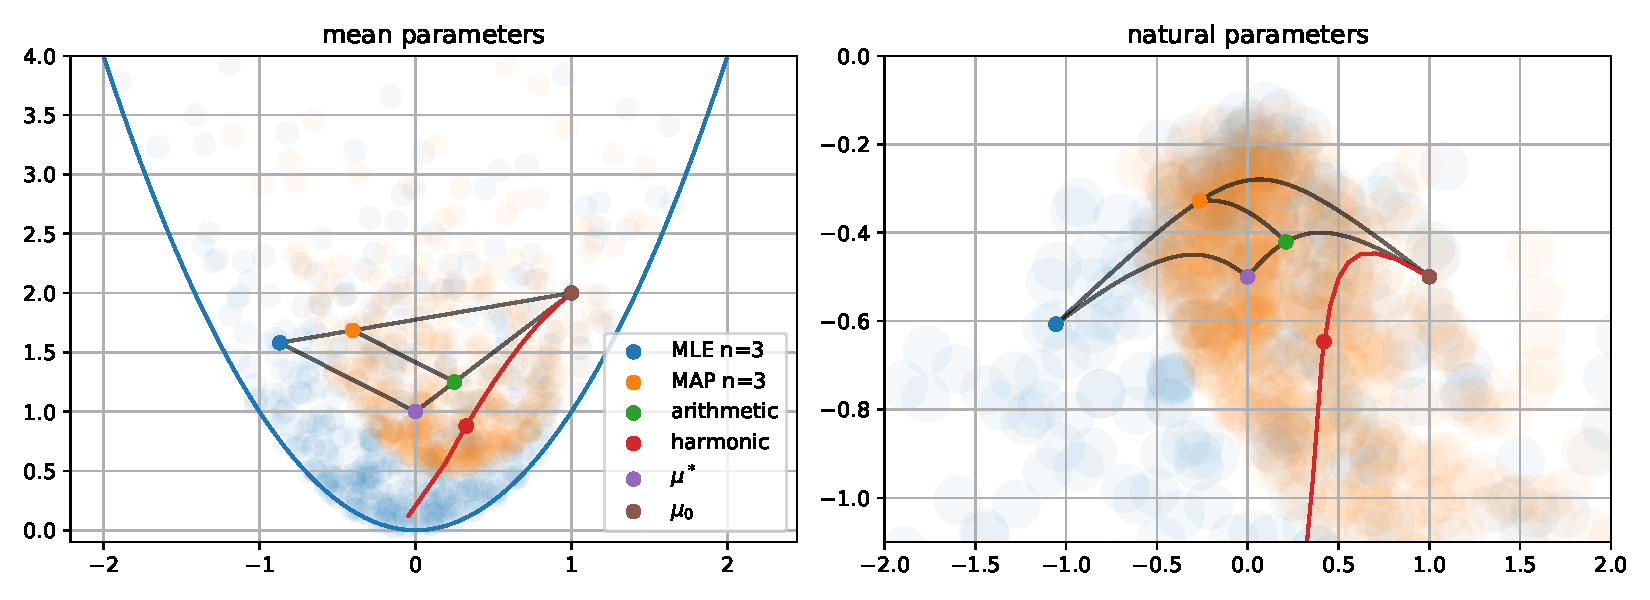
\includegraphics[width=\textwidth]{figs/thales/numerical_schema_n=3.pdf}
	\caption{A numerical illustration of the different characters featured in the bias-variance decomposition, for a 1D Gaussian $\cN(\mu, \sigma^2)$.}
	\label{fig:bias-variance-numerical}
\end{figure*}

\section{Bias-Variance Decomposition}
In both examples (add link), the upper bound takes the form $O(\inv{n}) + O(\frac{\text{bias}}{n^2})$, reminding us of the bias-variance decomposition. In fact, it is possible to write such a decomposition for any Bregman divergence
Let $\tilde \theta_n := \expect{\hat \theta_n}$ be the expectation of the MAP in primal space, and $\tilde \mu_n = \nabla \logpart(\tilde \theta_n )$ be the corresponding mean parameter.
As described by \citet[Theorem 0.1]{pfau2013generalized}, the  expected Bregman decomposes like
\begin{align}
	\expect{\bregmanconj(\mu^* ; \hat \mu_n)} 
	&= {\bregmanconj(\mu^* ; \tilde \mu_n)}
	+ {\expect{\bregmanconj(\tilde \mu_n ; \MAPm)}}
	\label{eq:primal_pivot}
\end{align}

\paragraph{Illustrations.}
We show these decompositions for $\cN(0,\sigma^2)$ in Figure~\ref{fig:variance_decomposition} and  $\cN(\mu, \sigma^2)$ in Figure~\ref{fig:gaussian_decomposition}.
In particular for $\cN(\mu, \sigma^2)$, we illustrate the characters featured in these decompositions $\hat \mu_n^\text{MLE},\hat \mu_n^\text{MAP},\mu_n,\tilde \mu_n, \mu^*$ and $\mu_0$ (and corresponding primal parameters)  in Figure~\ref{fig:bias-variance-numerical}. \RLP{Tune figures.}


\begin{figure*}[ht]
	\centering
	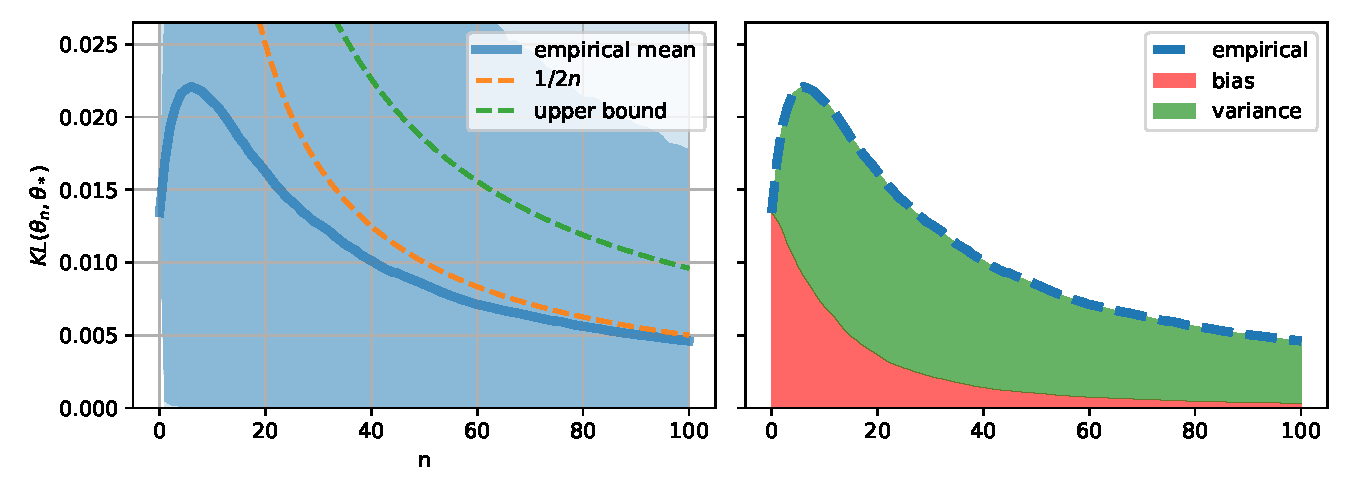
\includegraphics[width=\textwidth]{{figs/biasvariance/new_linear_ratio=0.8_n0=10}.pdf}
	\caption{
	\textbf{Gaussian variance $\cN(0,\sigma^2)$ example. Left:} training curves and analytic upper bound. 
	\textbf{Center:} bias-mixed-variance decomposition, using the arithmetic mean.
	\textbf{Right:} bias-variance decomposition, using the harmonic mean.
	}
	\label{fig:variance_decomposition}
\end{figure*}

\begin{figure*}[ht]
	\centering
	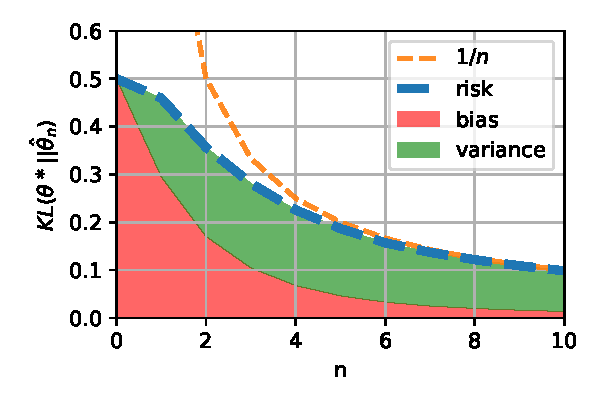
\includegraphics[width=\textwidth]{{figs/gaussians/new_linear_n0=1}.pdf}
	\caption{
	\textbf{Full gaussian} $\cN(m, \sigma^2)$ with $\meanp^*=(0, 1), \meanp_0 = (1,2)$ and $n_0=1$. \textbf{Left:} training curves (5,95) percentiles, average and asymptote. 
	\textbf{Right:} bias-variance decomposition.
	}
	\label{fig:gaussian_decomposition}
\end{figure*}








\section{Optimization related work}
In the context of optimization, why do we care? 

There is a long line work trying the convergence rate of stochastic gradient descent.
Beyond the results of RM51, 
we now have proofs n smooth, strongly convex problems and bounded variance 
(as well as other assumptions on the noise, reviewed later)
a decreasing step-size and an averaging scheme gets 
a $1/t$ convergence rate, 
which matches the asymptotic rate of unbiased estimation,
through clever averaging schemes \citep{rakhlin2012making,lacostejulien2012simpler}\footnote{
Those papers assume the stochastic gradients are bounded, 
but small modifications also work for bounded variance instead.
}

We do have extensions to other notions of bounded variance, 
for example assuming that the stochastic gradients are gradients of a perturbed smooth function $f_i$ 
and that the minimum of $f$ and the minima of the $f_i$ 
are bounded, $\expect{\min_x f(x) - \min_x f_i(x)} \leq \sigma^2$,
or that the gradient noise is bounded only at the minimum. 
For a review, see \citet{gower2019sgd}.

However, for some problems, combining decreasing step-sizes and averaging is not necessary,
even when the function is not strongly convex.
This is the case for maximum likelihood estimation and matches the asymptotic rates, 
but holds more generally, for example for linear and logistic regressions \citep{bach2013non}.

There has been recent advances in optimization that go beyond the Euclidean case, 
to optimize a function $f$ when it is not smooth, meaning its gradient is not $L$-Lipschitz,
neither strongly convex in the Euclidean norm, using the concept of relative smoothness 
\citep{bauschke2017descent,lu2018relatively},
where instead of measuring strong-convexity and smoothness relative to the Euclidean norm (or any norm), 
we use a reference function instead \fdk{maybe add a line}
and apply mirror descent \citep{nemirovski1983problem,beck2003mirror}
(also called NoLips \citep{bauschke2017descent}, something else?). 

We have convergence results for the 
application of stochastic mirror descent, 
but they typically rely on assumptions that are too strong. 
\begin{itemize}
	\item The reference function is strongly convex [typical setup in online learning]
	\item The variance is uniformly bounded
\end{itemize}
Some advances have been tried
\begin{itemize}
	\item The reference function is ``close to'' a norm
	and looks like a \citet{hanzely2018fastest}
	\item 
	Attempt to adapt the ``bounded gradient at the minimum''
	\citep{dragomir2021fast}
\end{itemize}

Other to cite;
\begin{itemize}
	\item \citet{marteauferey2019}
\end{itemize}


\fdk{
A ``simple open problem'';
assume we have a deterministic problem, so that we know where the minimum is. 
Can we figure out a (deterministic) path from $\theta_0$ to $\theta_*$ 
that has optimality decreasing as $1/n^2$, 
to mirror the bias term of gradient descent?
}


\fdk{
Application 

The problems on how to deal with Bregman divergences abound in optimization, beyond stochasticity. 
For example, we haven't yet figured out the analog of Nesterov-type acceleration 
on relatively smooth and strongly convex problems, 
to bring the convergence rate from linear in $(1-\kappa)$ to $(1-\sqrt{\kappa})$, 
or just from $1/T$ to $1/T^2$ 
in the (non-strongly) convex case.
\citet{dragomir2021optimal} show that naïve application of Bregman updates can not achieve acceleration.
The tools developped to make progress on one problem might help make progress on the other. 
}



	
	














\bibliographystyle{apalike}
\bibliography{../references.bib}




\clearpage
\section{Plan}

\begin{enumerate}
	\item intro to exponential family, and density estimation
	\item the thing we want to bound
	\item Examples : gaussian mean and gaussian variance (+other examples, just mentioned)
	\item Insight : Strongly convex case. (+ self-concordance that is not verified either)
	\item insight : bias-variance decomposition
	\item Optimization perspective : SBPP or SBG. But no analysis hold, revealing a flaw of all these techniques.
	\item Discussion : we believe finding a convergence rate would bring new tools useful to deal with common objects such as barrier losses.
\end{enumerate}

Open questions
\begin{itemize}
	\item does a base measure change anything ?
	\item is there multiple conjugate priors ?
	\item misspecified case. Do we have a   formula ?
\end{itemize}




\end{document}